\tikzset{every picture/.style={line width=0.75pt}} %set default line width to 0.75pt        

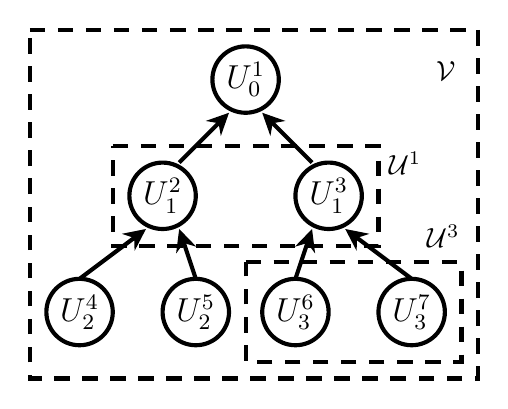
\begin{tikzpicture}[x=0.6pt,y=0.6pt,yscale=-1,xscale=1]
%uncomment if require: \path (0,300); %set diagram left start at 0, and has height of 300

%Shape: Circle [id:dp821654118938725] 
\draw  [line width=1.5]  (200,30) .. controls (200,18.95) and (208.95,10) .. (220,10) .. controls (231.05,10) and (240,18.95) .. (240,30) .. controls (240,41.05) and (231.05,50) .. (220,50) .. controls (208.95,50) and (200,41.05) .. (200,30) -- cycle ;
%Shape: Circle [id:dp7532382575897598] 
\draw  [line width=1.5]  (150,100) .. controls (150,88.95) and (158.95,80) .. (170,80) .. controls (181.05,80) and (190,88.95) .. (190,100) .. controls (190,111.05) and (181.05,120) .. (170,120) .. controls (158.95,120) and (150,111.05) .. (150,100) -- cycle ;
%Shape: Circle [id:dp5902978501813476] 
\draw  [line width=1.5]  (250,100) .. controls (250,88.95) and (258.95,80) .. (270,80) .. controls (281.05,80) and (290,88.95) .. (290,100) .. controls (290,111.05) and (281.05,120) .. (270,120) .. controls (258.95,120) and (250,111.05) .. (250,100) -- cycle ;
%Straight Lines [id:da9016881764549007] 
\draw [line width=1.5]    (207.17,52.83) -- (180,80) ;
\draw [shift={(210,50)}, rotate = 135] [fill={rgb, 255:red, 0; green, 0; blue, 0 }  ][line width=0.08]  [draw opacity=0] (13.4,-6.43) -- (0,0) -- (13.4,6.44) -- (8.9,0) -- cycle    ;
%Straight Lines [id:da026586992089503658] 
\draw [line width=1.5]    (232.83,52.83) -- (260,80) ;
\draw [shift={(230,50)}, rotate = 45] [fill={rgb, 255:red, 0; green, 0; blue, 0 }  ][line width=0.08]  [draw opacity=0] (13.4,-6.43) -- (0,0) -- (13.4,6.44) -- (8.9,0) -- cycle    ;
%Shape: Circle [id:dp7932559631044391] 
\draw  [line width=1.5]  (100,170) .. controls (100,158.95) and (108.95,150) .. (120,150) .. controls (131.05,150) and (140,158.95) .. (140,170) .. controls (140,181.05) and (131.05,190) .. (120,190) .. controls (108.95,190) and (100,181.05) .. (100,170) -- cycle ;
%Shape: Circle [id:dp8827895580667542] 
\draw  [line width=1.5]  (170,170) .. controls (170,158.95) and (178.95,150) .. (190,150) .. controls (201.05,150) and (210,158.95) .. (210,170) .. controls (210,181.05) and (201.05,190) .. (190,190) .. controls (178.95,190) and (170,181.05) .. (170,170) -- cycle ;
%Shape: Circle [id:dp1311962702995253] 
\draw  [line width=1.5]  (230,170) .. controls (230,158.95) and (238.95,150) .. (250,150) .. controls (261.05,150) and (270,158.95) .. (270,170) .. controls (270,181.05) and (261.05,190) .. (250,190) .. controls (238.95,190) and (230,181.05) .. (230,170) -- cycle ;
%Shape: Circle [id:dp055039676738894316] 
\draw  [line width=1.5]  (300,170) .. controls (300,158.95) and (308.95,150) .. (320,150) .. controls (331.05,150) and (340,158.95) .. (340,170) .. controls (340,181.05) and (331.05,190) .. (320,190) .. controls (308.95,190) and (300,181.05) .. (300,170) -- cycle ;
%Straight Lines [id:da3720861628053822] 
\draw [line width=1.5]    (156.8,122.4) -- (120,150) ;
\draw [shift={(160,120)}, rotate = 143.13] [fill={rgb, 255:red, 0; green, 0; blue, 0 }  ][line width=0.08]  [draw opacity=0] (13.4,-6.43) -- (0,0) -- (13.4,6.44) -- (8.9,0) -- cycle    ;
%Straight Lines [id:da5765340159287278] 
\draw [line width=1.5]    (181.26,123.79) -- (190,150) ;
\draw [shift={(180,120)}, rotate = 71.57] [fill={rgb, 255:red, 0; green, 0; blue, 0 }  ][line width=0.08]  [draw opacity=0] (13.4,-6.43) -- (0,0) -- (13.4,6.44) -- (8.9,0) -- cycle    ;
%Straight Lines [id:da8546030008258803] 
\draw [line width=1.5]    (258.74,123.79) -- (250,150) ;
\draw [shift={(260,120)}, rotate = 108.43] [fill={rgb, 255:red, 0; green, 0; blue, 0 }  ][line width=0.08]  [draw opacity=0] (13.4,-6.43) -- (0,0) -- (13.4,6.44) -- (8.9,0) -- cycle    ;
%Straight Lines [id:da21589979146129545] 
\draw [line width=1.5]    (283.2,122.4) -- (320,150) ;
\draw [shift={(280,120)}, rotate = 36.87] [fill={rgb, 255:red, 0; green, 0; blue, 0 }  ][line width=0.08]  [draw opacity=0] (13.4,-6.43) -- (0,0) -- (13.4,6.44) -- (8.9,0) -- cycle    ;
%Shape: Rectangle [id:dp24854624791356805] 
\draw  [dash pattern={on 5.63pt off 4.5pt}][line width=1.5]  (140,70) -- (300,70) -- (300,130) -- (140,130) -- cycle ;
%Shape: Rectangle [id:dp15950228071348826] 
\draw  [dash pattern={on 5.63pt off 4.5pt}][line width=1.5]  (220,140) -- (350,140) -- (350,200) -- (220,200) -- cycle ;
%Shape: Rectangle [id:dp8128591939925793] 
\draw  [dash pattern={on 5.63pt off 4.5pt}][line width=1.5]  (90,0) -- (360,0) -- (360,210) -- (90,210) -- cycle ;

% Text Node
\draw (340.5,25) node    {$\mathcal{V}$};
% Text Node
\draw (316,80.5) node    {$\mathcal{U}^{1}$};
% Text Node
\draw (339,124.5) node    {$\mathcal{U}^{3}$};
% Text Node
\draw (220,30) node  [font=\large]  {$U_{0}^{1}$};
% Text Node
\draw (170,100) node  [font=\large]  {$U_{1}^{2}$};
% Text Node
\draw (270,100) node  [font=\large]  {$U_{1}^{3}$};
% Text Node
\draw (120,170) node  [font=\large]  {$U_{2}^{4}$};
% Text Node
\draw (190,170) node  [font=\large]  {$U_{2}^{5}$};
% Text Node
\draw (250,170) node  [font=\large]  {$U_{3}^{6}$};
% Text Node
\draw (320,170) node  [font=\large]  {$U_{3}^{7}$};

\end{tikzpicture}
